%=====================================================================
%  SINDYc-MPC for RoSE v2.0 — Comprehensive Technical Notes
%  Colorful LaTeX document with equations, code, and hardware details
%=====================================================================
\documentclass[11pt,a4paper]{article}

%--- Packages ---
\usepackage[utf8]{inputenc}
\usepackage[T1]{fontenc}
\usepackage{lmodern}
\usepackage[margin=1in]{geometry}
\usepackage{amsmath,amssymb,bm}
\usepackage{graphicx}
\usepackage{xcolor}
\usepackage{hyperref}
\usepackage{listings}
\usepackage{booktabs}
\usepackage{enumitem}
\usepackage{tikz}
\usetikzlibrary{shapes.geometric, arrows.meta, positioning, calc, decorations.pathmorphing, patterns, fit}
\usepackage{tcolorbox}
\tcbuselibrary{listings, skins, breakable}
\usepackage{caption}
\usepackage{subcaption}
\usepackage{fancyhdr}
\usepackage{titlesec}

%--- Color Palette ---
\definecolor{rosepink}{HTML}{E91E63}
\definecolor{roseblue}{HTML}{1976D2}
\definecolor{rosegreen}{HTML}{388E3C}
\definecolor{roseorange}{HTML}{F57C00}
\definecolor{rosepurple}{HTML}{7B1FA2}
\definecolor{rosegray}{HTML}{455A64}
\definecolor{rosecyan}{HTML}{00838F}
\definecolor{roseteal}{HTML}{00695C}
\definecolor{lightblue}{HTML}{E3F2FD}
\definecolor{lightgreen}{HTML}{E8F5E9}
\definecolor{lightorange}{HTML}{FFF3E0}
\definecolor{lightpurple}{HTML}{F3E5F5}
\definecolor{lightpink}{HTML}{FCE4EC}
\definecolor{codebg}{HTML}{F5F5F5}

%--- Section Colors ---
\titleformat{\section}
  {\normalfont\Large\bfseries\color{roseblue}}
  {\thesection}{1em}{}
\titleformat{\subsection}
  {\normalfont\large\bfseries\color{rosepurple}}
  {\thesubsection}{1em}{}
\titleformat{\subsubsection}
  {\normalfont\normalsize\bfseries\color{roseteal}}
  {\thesubsubsection}{1em}{}

%--- Hyperlinks ---
\hypersetup{
    colorlinks=true,
    linkcolor=roseblue,
    urlcolor=rosepink,
    citecolor=rosegreen
}

%--- Code Listing Style ---
\lstdefinestyle{pythonstyle}{
    language=Python,
    backgroundcolor=\color{codebg},
    basicstyle=\ttfamily\footnotesize,
    keywordstyle=\color{roseblue}\bfseries,
    stringstyle=\color{rosegreen},
    commentstyle=\color{rosegray}\itshape,
    numberstyle=\tiny\color{rosegray},
    numbers=left,
    numbersep=6pt,
    frame=single,
    rulecolor=\color{rosegray!40},
    breaklines=true,
    showstringspaces=false,
    tabsize=4,
    morekeywords={self, np, ps, signal, minimize, True, False, None},
}
\lstset{style=pythonstyle}

%--- Colored Boxes ---
\newtcolorbox{conceptbox}[1][]{
    colback=lightblue,
    colframe=roseblue,
    fonttitle=\bfseries\color{white},
    coltitle=white,
    colbacktitle=roseblue,
    title={#1},
    breakable,
    enhanced,
    boxrule=0.8pt,
}
\newtcolorbox{equationbox}[1][]{
    colback=lightpurple,
    colframe=rosepurple,
    fonttitle=\bfseries\color{white},
    coltitle=white,
    colbacktitle=rosepurple,
    title={#1},
    breakable,
    enhanced,
    boxrule=0.8pt,
}
\newtcolorbox{hardwarebox}[1][]{
    colback=lightorange,
    colframe=roseorange,
    fonttitle=\bfseries\color{white},
    coltitle=white,
    colbacktitle=roseorange,
    title={#1},
    breakable,
    enhanced,
    boxrule=0.8pt,
}
\newtcolorbox{codebox}[1][]{
    colback=lightgreen,
    colframe=rosegreen,
    fonttitle=\bfseries\color{white},
    coltitle=white,
    colbacktitle=rosegreen,
    title={#1},
    breakable,
    enhanced,
    boxrule=0.8pt,
}
\newtcolorbox{warningbox}[1][]{
    colback=lightpink,
    colframe=rosepink,
    fonttitle=\bfseries\color{white},
    coltitle=white,
    colbacktitle=rosepink,
    title={#1},
    breakable,
    enhanced,
    boxrule=0.8pt,
}

%--- Header/Footer ---
\pagestyle{fancy}
\fancyhf{}
\fancyhead[L]{\small\textcolor{rosegray}{SINDYc-MPC for RoSE v2.0}}
\fancyhead[R]{\small\textcolor{rosegray}{Technical Notes}}
\fancyfoot[C]{\textcolor{rosegray}{\thepage}}

%=====================================================================
\begin{document}

\begin{titlepage}
\centering
\vspace*{0.5cm}

% --- Hardware cover image ---
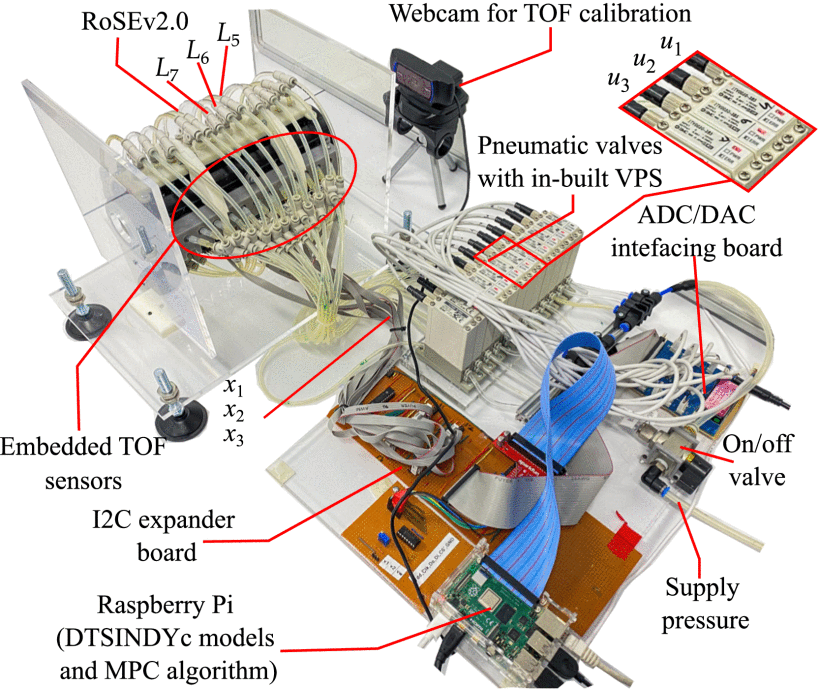
\includegraphics[width=0.85\textwidth]{figures/hardware_cover.png}

\vspace{0.8cm}

{\Huge\bfseries\textcolor{roseblue}{SINDYc-MPC for\\[0.3cm] RoSE v2.0 Peristaltic Soft Robot}\\[0.8cm]}
{\Large\textcolor{rosepurple}{Comprehensive Technical Notes}\\[0.4cm]}
{\large\textcolor{rosegray}{Discrete-Time Sparse Identification of Nonlinear Dynamics with Control\\
combined with Model Predictive Control}\\[1.2cm]}

% --- Author ---
{\Large \textbf{Dr~Dipankar Bhattacharya}\\[0.3cm]}
{\large\textcolor{rosegray}{Imperial College London}\\[1.5cm]}

% Pipeline Diagram
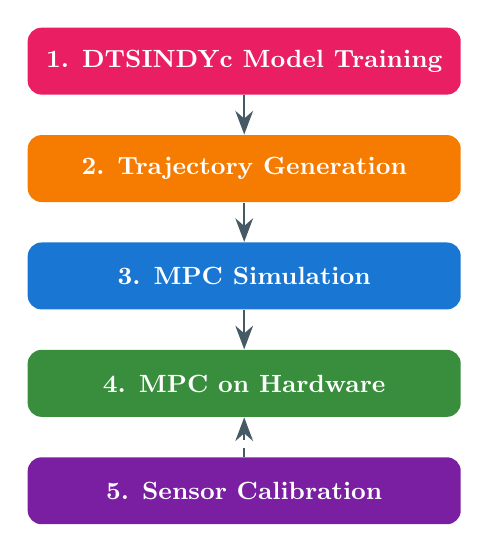
\begin{tikzpicture}[
    node distance=0.5cm,
    stage/.style={rectangle, rounded corners=5pt, minimum width=5.5cm, minimum height=0.85cm, text centered, font=\small\bfseries, text=white},
    arrow/.style={-{Stealth[length=3mm]}, thick, color=rosegray}
]
\node[stage, fill=rosepink]    (s1) {1. DTSINDYc Model Training};
\node[stage, fill=roseorange, below=of s1]  (s2) {2. Trajectory Generation};
\node[stage, fill=roseblue, below=of s2]    (s3) {3. MPC Simulation};
\node[stage, fill=rosegreen, below=of s3]   (s4) {4. MPC on Hardware};
\node[stage, fill=rosepurple, below=of s4]  (s5) {5. Sensor Calibration};

\draw[arrow] (s1) -- (s2);
\draw[arrow] (s2) -- (s3);
\draw[arrow] (s3) -- (s4);
\draw[arrow, dashed] (s5) -- (s4);
\end{tikzpicture}

\vfill
{\large\textcolor{rosegray}{Generated for the SINDYc\_MPC\_RoSE Project\\[0.3cm]}}
{\textcolor{rosegray}{\today}}
\end{titlepage}

\tableofcontents
\newpage

%=====================================================================
\section{Introduction and System Overview}
%=====================================================================

\begin{conceptbox}[What is RoSE v2.0?]
The \textbf{Robot of Soft Elastomer (RoSE) v2.0} is a 12-layer peristaltic soft robot
fabricated from silicone elastomer (Ecoflex 00-50). Each layer contains a pneumatic
chamber that can be independently inflated/deflated. By actuating layers in sequence
with phase-shifted sinusoidal signals, the robot produces \textbf{peristaltic locomotion}
--- a traveling wave contraction pattern similar to biological organisms.

The robot is instrumented with two types of embedded sensors:
\begin{itemize}[leftmargin=1.5cm]
    \item[\textcolor{roseblue}{\textbullet}] \textbf{VL6180X Time-of-Flight (TOF)} sensors --- measure layer displacement in mm
    \item[\textcolor{rosepink}{\textbullet}] \textbf{MCP3008 ADC / VPS} sensors --- measure internal pneumatic pressure in mV
\end{itemize}
\end{conceptbox}

\subsection{Control Objective}
The goal is to track a desired peristaltic wave trajectory across three monitored
layers (L5, L6, L7) using Model Predictive Control (MPC). The control pipeline is:

\begin{enumerate}
    \item \textbf{Learn} a data-driven discrete-time dynamic model (DTSINDYc)
    \item \textbf{Generate} a peristaltic wave reference trajectory
    \item \textbf{Optimize} control inputs using MPC with the learned model
    \item \textbf{Deploy} the controller on a Raspberry Pi in real time
\end{enumerate}

%=====================================================================
\section{Hardware Architecture}
\label{sec:hardware}
%=====================================================================

\subsection{System Block Diagram}

\begin{center}
\begin{figure}[h!]
    \centering
    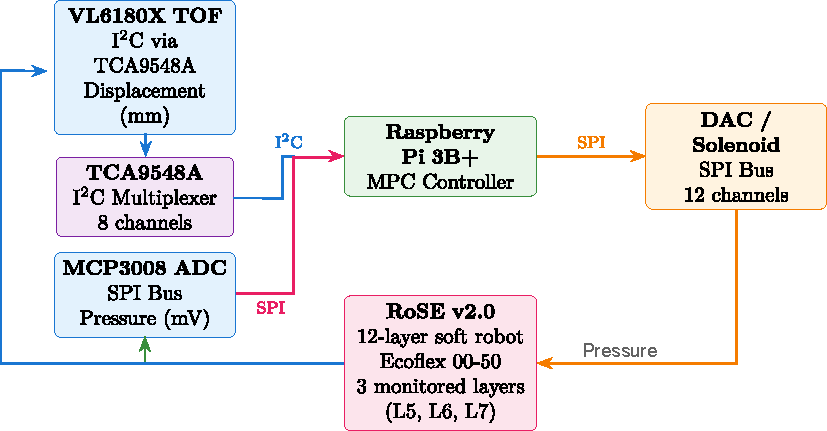
\includegraphics[width=0.8\textwidth]{figures/hardware_architecture.pdf}
    \caption{Hardware architecture of the RoSE v2.0 system. The Raspberry Pi interfaces with TOF sensors via an I$^2$C multiplexer and reads ADC values for pressure sensing. Control signals are sent to the pneumatic actuators through a DAC.}
    \label{fig:hardware_architecture}
\end{figure}
\end{center}

\subsection{VL6180X Time-of-Flight (TOF) Sensor}
\label{sec:tof}

\begin{hardwarebox}[TOF Sensor Specifications]
The \textbf{VL6180X} is a proximity/ambient light sensor from STMicroelectronics
that uses a VCSEL (Vertical-Cavity Surface-Emitting Laser) infrared emitter and
a SPAD (Single Photon Avalanche Diode) detector.

\begin{center}
\begin{tabular}{ll}
\toprule
\textbf{Parameter} & \textbf{Value} \\
\midrule
Measurement principle & Time-of-Flight (phase shift) \\
Range & 0--200 mm (effective: 5--100 mm) \\
Resolution & $\sim$1 mm \\
Interface & I$^2$C (default address: \texttt{0x29}) \\
Measurement rate & Up to 10 Hz (single-shot mode) \\
Supply voltage & 2.8 V \\
Field of view & 25$^\circ$ (cone) \\
\bottomrule
\end{tabular}
\end{center}

Since all VL6180X sensors share the same I$^2$C address (\texttt{0x29}), a
\textbf{TCA9548A} I$^2$C multiplexer is used to address each sensor on a
separate channel. The multiplexer supports 8 channels, of which 6 are used
for the 6 TOF sensors embedded in the robot.
\end{hardwarebox}

\subsubsection{TOF Calibration}
\label{sec:tofcal}

Each TOF sensor requires three calibration parameters:

\begin{equationbox}[TOF Calibration Model]
The calibrated displacement reading for sensor $i$ is:
\begin{equation}
    x_{\text{cal},i} = s_i \cdot (x_{\text{raw},i} - o_i) + b_i
    \label{eq:tof_cal}
\end{equation}
where:
\begin{itemize}
    \item $s_i$ --- scale factor (compensates for sensor-to-sensor gain variation)
    \item $o_i$ --- offset (compensates for mounting distance and crosstalk)
    \item $b_i$ --- baseline correction
\end{itemize}

\textbf{Typical calibration values:}
\begin{center}
\begin{tabular}{cccc}
\toprule
\textbf{Sensor} & \textbf{Scale $s_i$} & \textbf{Offset $o_i$} & \textbf{Baseline $b_i$} \\
\midrule
L5 & 0.72 & 23 & 1 \\
L6 & 0.67 & 73 & 0 \\
L7 & 0.32 & 69 & 1 \\
\bottomrule
\end{tabular}
\end{center}
\end{equationbox}

\begin{codebox}[TOF Sensor Reading --- Python Implementation]
\begin{lstlisting}
# From lib/ClassTOFandWebCam.py
def GenerateDisplacementDataFromTOF(self, t1):
    """Read displacement from 6 VL6180X ToF sensors"""
    return np.array([
        self.GenerateTimestamp(t1),
        self.TOF_sensor[0].range,  # Layer 5
        self.TOF_sensor[1].range,  # Layer 6
        self.TOF_sensor[2].range,  # Layer 7
        self.TOF_sensor[3].range,  # Layer 8
        self.TOF_sensor[4].range,  # Layer 9
        self.TOF_sensor[5].range   # Layer 10
    ])
\end{lstlisting}
\end{codebox}

\subsection{MCP3008 ADC Pressure Sensor}
\label{sec:adc}

\begin{hardwarebox}[ADC Sensor Specifications]
Pressure sensing uses \textbf{Voltage Proportional to Pressure Sensors (VPS)}
connected to an analog-to-digital converter.

\begin{center}
\begin{tabular}{ll}
\toprule
\textbf{Parameter} & \textbf{Value} \\
\midrule
ADC chip & MCP3008 (10-bit, 8 channels) \\
ADC alternate & MAXIM 11605 (8-bit, 12 channels) \\
Interface & SPI (MCP3008) / I$^2$C at \texttt{0x65} (MAXIM) \\
Channels monitored & 12 (3 primary: L5, L6, L7) \\
Measurement unit & mV $\to$ kPa (with calibration) \\
Sampling rate & Matched to control loop $T_s$ \\
\bottomrule
\end{tabular}
\end{center}

The ADC reads the voltage output of each VPS proportional to the pneumatic
pressure inside the corresponding silicone chamber.
\end{hardwarebox}

\begin{codebox}[ADC Pressure Reading --- Python Implementation]
\begin{lstlisting}
# From hardware MPC scripts
def GeneratePressureDataFromADC(self, NoOfADC=12):
    """Read 12 ADC channels via MAXIM 11605 ADC"""
    pressure_kpa_array = np.array([
        self.ADCbus.read_byte_data(
            self.ADC_ADDRESS,  # 0x65
            3 << 5 | i << 1 | 1
        ) for i in range(NoOfADC)
    ])
    return pressure_kpa_array
\end{lstlisting}
\end{codebox}

\subsection{Signal Conditioning --- FIR Low-Pass Filter}
\label{sec:filter}

Raw sensor readings are noisy. A \textbf{FIR (Finite Impulse Response)} low-pass
filter is applied in real time before feeding measurements to the controller.

\begin{equationbox}[FIR Filter Design]
The filter is designed using the Kaiser window method:
\begin{equation}
    y[n] = \sum_{k=0}^{M-1} b_k \cdot x[n-k]
    \label{eq:fir}
\end{equation}
where $b_k$ are the filter coefficients (FIR taps), $M$ is the filter order, and
$x[n]$ is the raw sensor measurement at sample $n$.

\textbf{Parameters:}
\begin{center}
\begin{tabular}{ll}
\toprule
\textbf{Parameter} & \textbf{Value} \\
\midrule
Number of taps $M$ & 10 \\
Normalized cutoff frequency & 0.1 (relative to Nyquist) \\
Window type & Kaiser / Hamming \\
\bottomrule
\end{tabular}
\end{center}
\end{equationbox}

\begin{codebox}[Real-Time FIR Filtering]
\begin{lstlisting}
numtaps_adc = 10
cutoff = 0.1  # Normalized cutoff
b_adc = signal.firwin(numtaps_adc, cutoff)
z_adc = signal.lfilter_zi(b_adc, 1)

# Apply in real-time (per sample)
x_filtered, z_adc = signal.lfilter(
    b_adc, 1, [x_raw_measurement], zi=z_adc
)
\end{lstlisting}
\end{codebox}

%=====================================================================
\section{Stage 1 --- DTSINDYc Model Training}
\label{sec:sindy}
%=====================================================================

\begin{conceptbox}[What is SINDYc?]
\textbf{Sparse Identification of Nonlinear Dynamics with control (SINDYc)} is a
data-driven method that discovers governing equations from measurement data.
Instead of assuming a model structure, SINDYc builds a \emph{library} of
candidate functions and uses sparse regression to select only the terms that
are active --- yielding an interpretable, parsimonious model.

The \textbf{discrete-time} variant (DTSINDYc) discovers difference equations:
\[
    \mathbf{x}_{k+1} = f(\mathbf{x}_k, \mathbf{u}_k)
\]
directly from sampled sensor data, avoiding numerical differentiation entirely.
\end{conceptbox}

\subsection{Mathematical Formulation}

\subsubsection{State and Control Vectors}

The robot state $\mathbf{x} \in \mathbb{R}^3$ and control input $\mathbf{u} \in \mathbb{R}^3$
are measured at three layers:

\begin{equationbox}[State and Control Definitions]
\textbf{Model M1 (TOF-based):}
\begin{equation}
    \mathbf{x}_k^{\text{TOF}} = \begin{bmatrix} d_{L5}(t_k) \\ d_{L6}(t_k) \\ d_{L7}(t_k) \end{bmatrix} \in \mathbb{R}^3
    \quad\text{(displacement in mm)}
    \label{eq:state_tof}
\end{equation}

\textbf{Model M2 (ADC/VPS-based):}
\begin{equation}
    \mathbf{x}_k^{\text{ADC}} = \begin{bmatrix} p_{L5}(t_k) \\ p_{L6}(t_k) \\ p_{L7}(t_k) \end{bmatrix} \in \mathbb{R}^3
    \quad\text{(pressure in mV)}
    \label{eq:state_adc}
\end{equation}

\textbf{Control input (shared):}
\begin{equation}
    \mathbf{u}_k = \begin{bmatrix} v_{L5}(t_k) \\ v_{L6}(t_k) \\ v_{L7}(t_k) \end{bmatrix} \in \mathbb{R}^3
    \quad\text{(DAC voltage command)}
    \label{eq:control}
\end{equation}
\end{equationbox}

\subsubsection{Polynomial Library Construction}

\begin{equationbox}[Candidate Function Library $\bm{\Theta}$]
Given state $\mathbf{x} = [x_1, x_2, x_3]^T$ and control $\mathbf{u} = [u_1, u_2, u_3]^T$,
the polynomial library of degree $p=2$ is:
\begin{equation}
    \bm{\Theta}(\mathbf{x}_k, \mathbf{u}_k) = \Big[\underbrace{1}_{\text{const}},\;
    \underbrace{x_1, x_2, x_3}_{\text{states}},\;
    \underbrace{u_1, u_2, u_3}_{\text{controls}},\;
    \underbrace{x_1^2, x_1 x_2, \ldots, u_3^2}_{\text{quadratic}}\Big]
    \label{eq:library}
\end{equation}
For $n=6$ variables (3 states + 3 controls) and degree $p=2$, the library contains:
\[
    \binom{n+p}{p} = \binom{8}{2} = 28 \text{ candidate terms}
\]
\end{equationbox}

\begin{codebox}[Library Construction --- \texttt{sindybase.py}]
\begin{lstlisting}
def polynomial_expansion(self, data, degree=2):
    """
    Expands [x1, x2, x3, u1, u2, u3] into all
    polynomial combinations up to specified degree.
    """
    nfeat = data.shape[-1]  # 6 (states + controls)
    exponents = SINDyBase.get_ordered_poly_exponents(
        nfeat, degree
    )
    result = np.array([
        np.prod(
            [data[:, k] ** e[k] for k in range(nfeat)],
            axis=0
        ) for e in exponents
    ]).T
    return result  # Shape: (T, 28) for degree=2
\end{lstlisting}
\end{codebox}

\subsubsection{Sparse Regression (STLSQ)}

\begin{equationbox}[Sequential Thresholded Least Squares (STLSQ)]
The DTSINDYc model is:
\begin{equation}
    \mathbf{x}_{k+1} = \bm{\Theta}(\mathbf{x}_k, \mathbf{u}_k) \,\bm{\Xi}
    \label{eq:sindy_model}
\end{equation}
where $\bm{\Xi} \in \mathbb{R}^{28 \times 3}$ is the sparse coefficient matrix.

$\bm{\Xi}$ is found by solving the sparse regression problem:
\begin{equation}
    \min_{\bm{\Xi}} \left\| \mathbf{X}_{k+1} - \bm{\Theta}_k \bm{\Xi} \right\|_2^2
    \quad\text{subject to}\quad \|\bm{\Xi}\|_0 \text{ is small}
    \label{eq:stlsq_objective}
\end{equation}

\textbf{STLSQ Algorithm:}
\begin{enumerate}
    \item Solve the least-squares problem: $\bm{\Xi}^{(0)} = (\bm{\Theta}^T\bm{\Theta})^{-1}\bm{\Theta}^T \mathbf{X}_{k+1}$
    \item For each iteration $j = 1, \ldots, j_{\max}$:
    \begin{enumerate}
        \item Set $\Xi_{ij}^{(j)} = 0$ if $|\Xi_{ij}^{(j-1)}| \leq \lambda$ \quad {\small\textcolor{rosepink}{(threshold sparsification)}}
        \item Re-solve least squares on remaining (non-zero) coefficients
    \end{enumerate}
    \item Return $\bm{\Xi}^{(j_{\max})}$
\end{enumerate}

\textbf{Parameters:}
\begin{center}
\begin{tabular}{lll}
\toprule
\textbf{Symbol} & \textbf{Parameter} & \textbf{Value} \\
\midrule
$\lambda$ & Sparsification threshold & 0.008 \\
$\alpha$ & Regularization (L2 penalty) & 0.5 \\
$p$ & Polynomial degree & 2 \\
$j_{\max}$ & Maximum STLSQ iterations & 10 \\
\bottomrule
\end{tabular}
\end{center}
\end{equationbox}

\begin{codebox}[STLSQ Implementation --- \texttt{sindybase.py}]
\begin{lstlisting}
@staticmethod
def threshold_ls(mtx, _b, lam_bda=1e-3, max_iter=10):
    """
    Sparse regression via sequential thresholding.
    mtx: library Theta (M x 28)
    _b:  next-state data X_{k+1} (M x 3)
    lam_bda: sparsification threshold
    """
    # Step 1: Initial least-squares
    _w = np.linalg.lstsq(mtx, _b, rcond=None)[0]

    # Step 2: Iterative thresholding
    for _ in range(max_iter):
        small_inds = np.abs(_w) <= lam_bda
        _w[small_inds] = 0  # Kill small coefficients

        for ind in range(_b.shape[1]):
            big_inds = ~small_inds[:, ind]
            _w[big_inds, ind] = np.linalg.lstsq(
                mtx[:, big_inds], _b[:, ind],
                rcond=None
            )[0]
    return _w
\end{lstlisting}
\end{codebox}

\subsubsection{PySINDy Model Fitting}

\begin{codebox}[Training a DTSINDYc Model with PySINDy]
\begin{lstlisting}
import pysindy as ps

# Configure optimizer
stlsq_optimizer = ps.STLSQ(
    threshold=0.008,  # lambda
    alpha=0.5         # L2 regularization
)

# Configure polynomial library (degree 2)
poly_library = ps.PolynomialLibrary(
    include_interaction=True,
    interaction_only=False,
    degree=2
)

# Create and fit DTSINDYc model
model = ps.SINDy(
    optimizer=stlsq_optimizer,
    feature_library=poly_library
)

# Discrete-time fitting: x[k+1] = f(x[k], u[k])
model.fit(
    x_train[:-1],       # States at time k
    x_dot=x_train[1:],  # States at time k+1
    u=u_train[:-1]       # Controls at time k
)

model.print()
# Example output for 1-state symmetric:
# (x0)' = 0.812 + 0.985 x0 + 0.189 u0 - 0.003 x0*u0
\end{lstlisting}
\end{codebox}

\begin{warningbox}[Discovered Model Example --- 1-State Symmetric (M2/ADC)]
For the 1-state symmetric actuation (all layers move in unison), the DTSINDYc
model discovers:
\begin{equation}
    x_{k+1} = \underset{\text{bias}}{0.812} + \underset{\text{autoregressive}}{0.985\, x_k}
    + \underset{\text{control gain}}{0.189\, u_k}
    - \underset{\text{nonlinear coupling}}{0.003\, x_k u_k}
    \label{eq:discovered_model}
\end{equation}
The sparse regression has retained only 4 of 28 candidate terms --- a parsimonious
model that captures the dominant dynamics.
\end{warningbox}

%=====================================================================
\section{Stage 2 --- Reference Trajectory Generation}
\label{sec:trajectory}
%=====================================================================

\begin{conceptbox}[Peristaltic Wave]
Peristalsis is a traveling wave of contraction and relaxation. For the RoSE robot,
this is achieved by actuating successive layers with a phase-shifted sinusoidal
signal. The wave propagates along the robot body, producing forward locomotion.
\end{conceptbox}

\subsection{Mathematical Definition}

\begin{equationbox}[Peristaltic Reference Trajectory (Eq.\ 14 in Paper)]
The reference displacement for layer $i$ at time step $t$ is:
\begin{equation}
    h_i(t) = \begin{cases}
        \epsilon & \text{if } t \leq n_i \cdot \delta \\[6pt]
        \epsilon + \dfrac{\alpha}{2}\left(1 - \cos\!\left(\dfrac{2\pi(n_i \cdot \delta - t)}{\lambda_d}\right)\right) & \text{if } n_i \cdot \delta < t < n_i \cdot \delta + \lambda_d \\[6pt]
        \epsilon & \text{if } t \geq n_i \cdot \delta + \lambda_d
    \end{cases}
    \label{eq:peristaltic_ref}
\end{equation}
where:
\begin{center}
\begin{tabular}{lll}
\toprule
\textbf{Symbol} & \textbf{Description} & \textbf{Value} \\
\midrule
$\alpha$ & Wave amplitude & 10 (mm or mV) \\
$\epsilon$ & Baseline offset & 0 \\
$\lambda_d$ & Wavelength in samples & $\lambda_{\text{time}} / T_s = 6 / 0.35 \approx 17$ \\
$\delta$ & Propagation delay in samples & $\Delta t_{\text{prop}} / T_s = (15/18.75) / 0.35 \approx 2.3$ \\
$n_i$ & Layer index (0, 1, 2) & L5 $\to$ 0, L6 $\to$ 1, L7 $\to$ 2 \\
$T_s$ & Sampling period & 0.35 s \\
\bottomrule
\end{tabular}
\end{center}
\end{equationbox}

\subsection{Phase-Shifted Three-Channel Wave}

\begin{center}
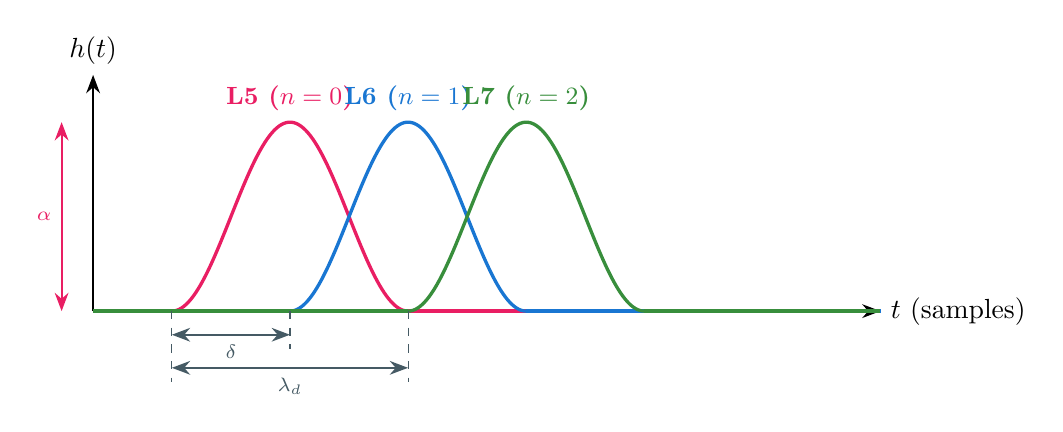
\begin{tikzpicture}[xscale=0.5, yscale=0.6]
    % Axes
    \draw[-{Stealth}, thick] (0,0) -- (20,0) node[right] {$t$ (samples)};
    \draw[-{Stealth}, thick] (0,0) -- (0,5) node[above] {$h(t)$};

    % Channel 0 (L5) - no delay
    \draw[very thick, rosepink, domain=0:2, samples=50] plot (\x, 0);
    \draw[very thick, rosepink, domain=2:8, samples=100]
        plot (\x, {2*(1-cos(180*(\x-2)/3))});
    \draw[very thick, rosepink, domain=8:20, samples=50] plot (\x, 0);
    \node[rosepink, font=\small\bfseries] at (5, 4.5) {L5 ($n=0$)};

    % Channel 1 (L6) - 1x delay
    \draw[very thick, roseblue, domain=0:5, samples=50] plot (\x, 0);
    \draw[very thick, roseblue, domain=5:11, samples=100]
        plot (\x, {2*(1-cos(180*(\x-5)/3))});
    \draw[very thick, roseblue, domain=11:20, samples=50] plot (\x, 0);
    \node[roseblue, font=\small\bfseries] at (8, 4.5) {L6 ($n=1$)};

    % Channel 2 (L7) - 2x delay
    \draw[very thick, rosegreen, domain=0:8, samples=50] plot (\x, 0);
    \draw[very thick, rosegreen, domain=8:14, samples=100]
        plot (\x, {2*(1-cos(180*(\x-8)/3))});
    \draw[very thick, rosegreen, domain=14:20, samples=50] plot (\x, 0);
    \node[rosegreen, font=\small\bfseries] at (11, 4.5) {L7 ($n=2$)};

    % Annotations
    \draw[{Stealth}-{Stealth}, thick, rosegray] (2,-0.5) -- node[below, font=\scriptsize] {$\delta$} (5,-0.5);
    \draw[{Stealth}-{Stealth}, thick, rosegray] (2,-1.2) -- node[below, font=\scriptsize] {$\lambda_d$} (8,-1.2);
    \draw[dashed, rosegray] (2,0) -- (2,-1.5);
    \draw[dashed, rosegray] (5,0) -- (5,-0.8);
    \draw[dashed, rosegray] (8,0) -- (8,-1.5);

    % Amplitude annotation
    \draw[{Stealth}-{Stealth}, thick, rosepink] (-0.8, 0) -- node[left, font=\scriptsize] {$\alpha$} (-0.8, 4);
\end{tikzpicture}
\end{center}
\captionof{figure}{Three-channel peristaltic wave reference trajectory. Each layer is
phase-shifted by $\delta$ samples, creating a traveling wave.}

\begin{codebox}[Trajectory Generation Code]
\begin{lstlisting}
Ts = 0.35              # Sampling period (s)
lamb_time = 6          # Wavelength time period (s)
lamb_dis = int(lamb_time / Ts)  # ~17 samples
alpha = 10             # Amplitude
epsilon = 0            # Baseline offset
delay = int((15 / 18.75) / Ts)  # ~2 samples

H = np.zeros((total_samples, 3))

for i, t in enumerate(time_steps):
    for ch in range(3):  # 3 layers
        d_ch = ch * delay  # Phase delay
        if t <= d_ch:
            H[i, ch] = epsilon
        elif t >= d_ch + lamb_dis:
            H[i, ch] = epsilon
        else:
            H[i, ch] = epsilon + (alpha / 2) * (
                1 - np.cos(2*np.pi*(d_ch - t) / lamb_dis)
            )
\end{lstlisting}
\end{codebox}

%=====================================================================
\section{Stage 3 --- Model Predictive Control (MPC)}
\label{sec:mpc}
%=====================================================================

\begin{conceptbox}[Nonlinear MPC with DTSINDYc Model]
The MPC controller uses the identified DTSINDYc model (Eq.~\ref{eq:sindy_model})
as a predictor to optimize future control actions. At each time step $k$, it
solves a constrained optimization problem over a prediction horizon $N$, applies
only the first control action, then re-solves at $k+1$ (receding horizon).
\end{conceptbox}

\subsection{MPC Cost Function}

\begin{equationbox}[MPC Optimization Problem]
At each time step $k$, solve:
\begin{equation}
    \min_{\mathbf{u}_k, \ldots, \mathbf{u}_{k+N-1}} \; J = \sum_{j=0}^{N-1} \Big[
        \underbrace{(\mathbf{x}_{k+j+1} - \mathbf{x}_{\text{ref}})^T \mathbf{Q}\, (\mathbf{x}_{k+j+1} - \mathbf{x}_{\text{ref}})}_{\text{tracking error}}
    + \underbrace{(\Delta\mathbf{u}_{k+j})^T \mathbf{R}\, \Delta\mathbf{u}_{k+j}}_{\text{control variation}}
    + \underbrace{\mathbf{u}_{k+j}^T \mathbf{R}_u\, \mathbf{u}_{k+j}}_{\text{control effort}}
    \Big]
    \label{eq:mpc_cost}
\end{equation}
subject to:
\begin{align}
    \mathbf{x}_{k+j+1} &= \bm{\Theta}(\mathbf{x}_{k+j}, \mathbf{u}_{k+j})\,\bm{\Xi}
    && \text{(DTSINDYc model constraint)} \label{eq:mpc_dynamics} \\
    \mathbf{u}_{\min} &\leq \mathbf{u}_{k+j} \leq \mathbf{u}_{\max}
    && \text{(actuator bounds)} \label{eq:mpc_bounds}
\end{align}
where $\Delta\mathbf{u}_{k+j} = \mathbf{u}_{k+j} - \mathbf{u}_{k+j-1}$ is the control increment.
\end{equationbox}

\subsection{Weight Matrices and Parameters}

\begin{equationbox}[MPC Tuning Parameters]
\begin{center}
\begin{tabular}{lll}
\toprule
\textbf{Symbol} & \textbf{Description} & \textbf{Value} \\
\midrule
$\mathbf{Q}$ & State tracking weight & $\text{diag}(5,\; 10,\; 5)$ \\
$\mathbf{R}$ & Control variation weight & $\text{diag}(0.5,\; 0.5,\; 0.5)$ \\
$\mathbf{R}_u$ & Control effort weight & $\text{diag}(0.5,\; 0.5,\; 0.5)$ \\
$N$ & Prediction horizon & 4 (also tested: 1, 2) \\
$T_s$ & Sampling time & 0.5 s \\
Solver & Optimization method & SLSQP \\
$\text{tol}$ & Convergence tolerance & 0.1 \\
\bottomrule
\end{tabular}
\end{center}

\textbf{Note:} The higher weight on $x_2$ (layer L6, $Q_{22}=10$) reflects that the
center layer is more critical for peristaltic wave shape accuracy.
\end{equationbox}

\subsection{State-Dependent Control Constraints}

The actuator bounds are adaptive, depending on the current reference level:

\begin{equationbox}[Dynamic Bounds for Channel 1]
\begin{equation}
    (u_{\min,1},\; u_{\max,1}) = \begin{cases}
        (40,\; 46) & \text{if } x_{\text{ref},1} \geq 7.6 \\
        (32,\; 40) & \text{if } 5.5 \leq x_{\text{ref},1} < 7.6 \\
        (24,\; 32) & \text{if } 2.0 \leq x_{\text{ref},1} < 5.5 \\
        (9,\; 17)  & \text{if } x_{\text{ref},1} < 2.0
    \end{cases}
    \label{eq:bounds}
\end{equation}
Similar adaptive bounds apply to channels 2 and 3. This schedule
prevents excessive actuation and ensures the optimization stays near
the operating region where the SINDy model is valid.
\end{equationbox}

\begin{codebox}[MPC Objective Function Implementation]
\begin{lstlisting}
def RobotObjectiveFCN(self, u, *args):
    x, Ts, N, xref, u0, Q, R, Ru = args
    xk = x
    u = u.reshape((3, -1))  # (3 channels, N steps)
    J = 0

    for kk in range(N):
        uk = u[:, kk]
        # Predict next state via SINDy model
        xk1 = self.model.predict(
            xk[np.newaxis, :], uk[np.newaxis, :]
        )[0, :]

        # Tracking cost
        e = xk1 - xref
        J += e.T @ Q @ e

        # Control variation cost
        du = uk - (u0 if kk == 0 else u[:, kk-1])
        J += du.T @ R @ du

        # Control effort cost
        J += uk.T @ Ru @ uk

        xk = xk1  # Propagate state
    return J
\end{lstlisting}
\end{codebox}

\subsection{MPC Block Diagram}

\begin{center}
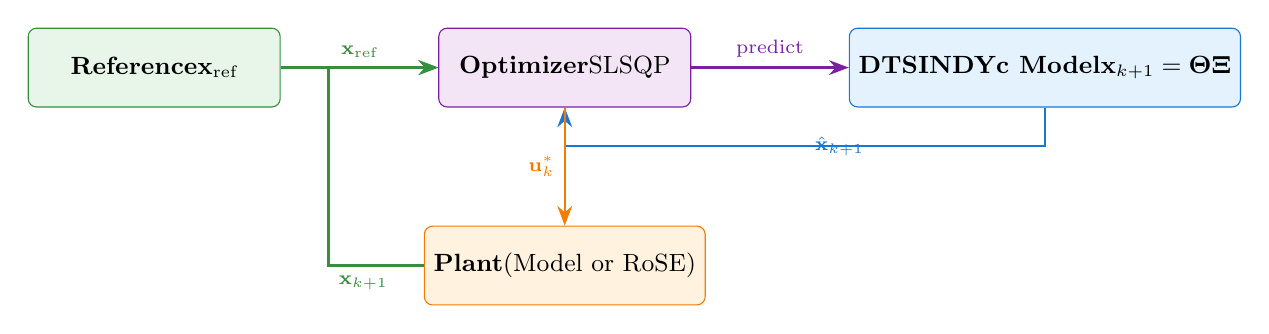
\begin{tikzpicture}[
    block/.style={rectangle, draw, rounded corners=3pt, minimum width=3.2cm, minimum height=1cm, text centered, font=\small},
    arr/.style={-{Stealth[length=2.5mm]}, thick},
    node distance=1.2cm
]
\node[block, fill=lightpurple, draw=rosepurple] (opt) {\textbf{Optimizer}\\SLSQP};
\node[block, fill=lightblue, draw=roseblue, right=2cm of opt] (model) {\textbf{DTSINDYc Model}\\$\mathbf{x}_{k+1} = \bm{\Theta}\bm{\Xi}$};
\node[block, fill=lightorange, draw=roseorange, below=1.5cm of opt] (plant) {\textbf{Plant}\\(Model or RoSE)};
\node[block, fill=lightgreen, draw=rosegreen, left=2cm of opt] (ref) {\textbf{Reference}\\$\mathbf{x}_{\text{ref}}$};

\draw[arr, rosepurple] (opt) -- node[above, font=\scriptsize] {predict} (model);
\draw[arr, roseblue] (model) -- ++(0,-1) -| node[near start, right, font=\scriptsize] {$\hat{\mathbf{x}}_{k+1}$} (opt);
\draw[arr, roseorange] (opt) -- node[left, font=\scriptsize] {$\mathbf{u}_k^*$} (plant);
\draw[arr, rosegreen] (plant) -| node[below right, font=\scriptsize] {$\mathbf{x}_{k+1}$} ++(-3, 0) |- (opt);
\draw[arr, rosegreen] (ref) -- node[above, font=\scriptsize] {$\mathbf{x}_{\text{ref}}$} (opt);
\end{tikzpicture}
\end{center}
\captionof{figure}{MPC receding-horizon control loop. At each step, the optimizer uses
the DTSINDYc model to predict future states and find the optimal control sequence.}

%=====================================================================
\section{Stage 4 --- Real-Time MPC on Hardware}
\label{sec:hardware_mpc}
%=====================================================================

\subsection{Control Loop Architecture}

\begin{center}
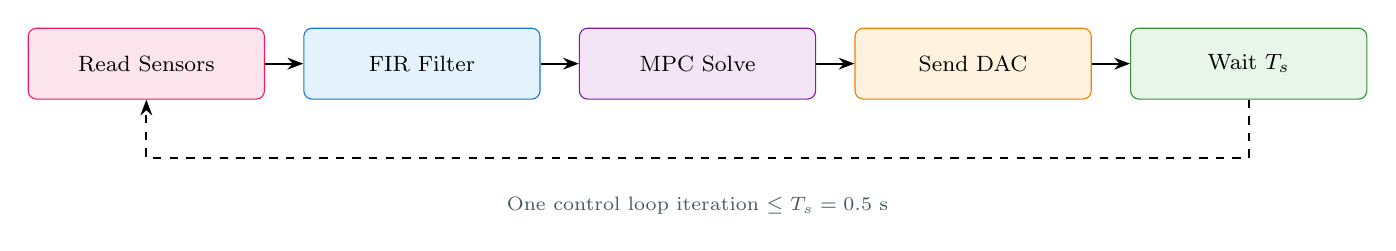
\begin{tikzpicture}[
    block/.style={rectangle, draw, rounded corners=3pt, minimum width=3cm, minimum height=0.9cm, text centered, font=\footnotesize},
    arr/.style={-{Stealth[length=2mm]}, thick},
    every node/.style={font=\small}
]
% Timeline
\node[block, fill=lightpink, draw=rosepink] (read) at (0,0) {Read Sensors};
\node[block, fill=lightblue, draw=roseblue] (filter) at (3.5,0) {FIR Filter};
\node[block, fill=lightpurple, draw=rosepurple] (mpc) at (7,0) {MPC Solve};
\node[block, fill=lightorange, draw=roseorange] (send) at (10.5,0) {Send DAC};
\node[block, fill=lightgreen, draw=rosegreen] (wait) at (14,0) {Wait $T_s$};

\draw[arr] (read) -- (filter);
\draw[arr] (filter) -- (mpc);
\draw[arr] (mpc) -- (send);
\draw[arr] (send) -- (wait);
\draw[arr, dashed] (wait) |- ++(0,-1.2) -| (read);

% Timing
\node[rosegray, font=\scriptsize] at (7,-1.8) {One control loop iteration $\leq T_s = 0.5$ s};
\end{tikzpicture}
\end{center}

\begin{codebox}[Real-Time MPC Loop on Raspberry Pi]
\begin{lstlisting}
for ct in range(int(Duration / Ts)):
    t_start = time.time()

    # 1. Read sensors
    tof_data = self.GenerateDisplacementDataFromTOF(t1)
    adc_data = self.GeneratePressureDataFromADC(12)

    # 2. Apply FIR filter
    x_filtered, z = Filter_RealTime_apply(
        tof_data[1:4], b_filter, z
    )

    # 3. Get reference for current time step
    xref = xref_trajectory[:, ct]

    # 4. Compute adaptive bounds from xref
    bounds = compute_adaptive_bounds(xref)

    # 5. Solve MPC optimization (SLSQP)
    result = minimize(
        self.RobotObjectiveFCN, u_prev,
        method='SLSQP',
        args=(x_filtered, Ts, N, xref, u0, Q, R, Ru),
        tol=0.1, bounds=bounds
    )
    u_optimal = result.x[:3]  # First step only

    # 6. Send control to 12-layer actuator array
    self.mergeDACadd2DataAndSend(
        u_optimal, 0, BaseLinePress, ScalingFact
    )

    # 7. Wait for next sampling instant
    elapsed = time.time() - t_start
    if elapsed < Ts:
        time.sleep(Ts - elapsed)
\end{lstlisting}
\end{codebox}

\subsection{3-State to 12-Layer Mapping}

The MPC computes 3 control signals (one per monitored layer), but the robot has
12 actuatable layers. The 3 MPC outputs are mapped to all 12 layers using a
rotating deque pattern that propagates the peristaltic wave:

\begin{equationbox}[Layer Mapping for Peristaltic Actuation]
\begin{equation}
    \mathbf{u}_{\text{12-layer}}[k] = \mathcal{R}^k\!\left(\begin{bmatrix}
        u_1 & u_1 & u_1 & u_1 & u_2 & u_2 & u_2 & u_2 & u_3 & u_3 & u_3 & u_3
    \end{bmatrix}\right)
    \label{eq:layer_mapping}
\end{equation}
where $\mathcal{R}^k$ denotes a circular shift (rotation) by $k \cdot 3$ positions,
creating the traveling wave pattern across the full 12-layer robot body.
\end{equationbox}

%=====================================================================
\section{Stage 5 --- Sensor Calibration}
\label{sec:calibration}
%=====================================================================

\begin{conceptbox}[Why Calibrate?]
Raw sensor readings suffer from:
\begin{itemize}
    \item \textbf{Offset errors} --- mounting distance introduces a constant bias
    \item \textbf{Crosstalk} --- adjacent TOF sensors interfere (IR reflections)
    \item \textbf{Gain variation} --- each VL6180X has slightly different responsivity
    \item \textbf{Convergence time} --- sensors need warm-up for stable readings
\end{itemize}
Calibration must be performed \emph{before} collecting training data or deploying MPC.
\end{conceptbox}

\subsection{TOF Calibration Procedure}

The calibration script (\texttt{5\_hardware\_calibration/}) performs:

\begin{enumerate}
    \item \textbf{Offset calibration}: Place a known target at a reference distance.
    Record the raw reading and compute $o_i = x_{\text{raw}} - x_{\text{true}}$.
    \item \textbf{Scale factor}: Measure at multiple known distances. Fit a linear model
    $x_{\text{true}} = s_i \cdot x_{\text{raw}} + c_i$ via least squares.
    \item \textbf{Crosstalk compensation}: Fire one sensor at a time and record
    readings on neighboring sensors. Subtract the crosstalk component.
    \item \textbf{Convergence time}: Record sensor output after power-on and determine
    the settling time before readings stabilize (typically 1--2 s).
\end{enumerate}

\subsection{ADC Calibration (Full-Scale Pressure)}

The MCP3008 ADC is calibrated using a known pressure source:

\begin{equationbox}[ADC Full-Scale Calibration]
\begin{equation}
    p_{\text{cal}} = \frac{V_{\text{ADC}}}{V_{\text{ref}}} \times p_{\text{full-scale}}
    \label{eq:adc_cal}
\end{equation}
where $V_{\text{ref}} = 3.3$ V (Raspberry Pi reference voltage) and
$p_{\text{full-scale}}$ is determined by the VPS sensor datasheet.
The script \texttt{Mcp3008\_FSP\_Cal.py} automates this process.
\end{equationbox}

%=====================================================================
\section{Data Flow and Directory Map}
\label{sec:dataflow}
%=====================================================================
\begin{center}
\begin{figure}[h!]
    \centering
    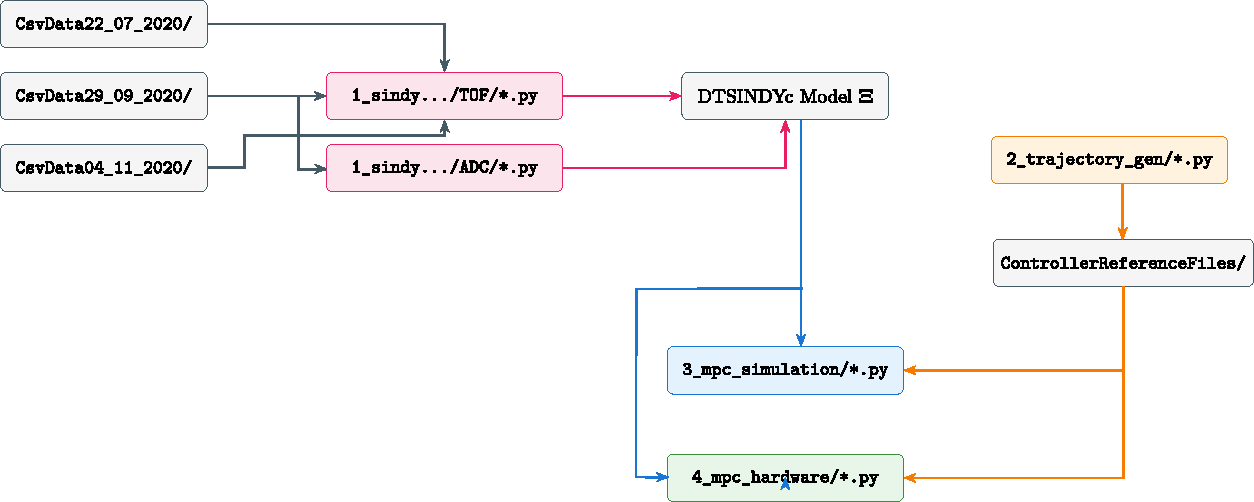
\includegraphics[width=0.8\textwidth]{figures/sim_exp_block_diagram.pdf}
    \caption{Data flow across the pipeline stages. CSV experimental data feeds
into model training (Stage 1), which produces the DTSINDYc model used by both
MPC simulation (Stage 3) and hardware deployment (Stage 4).}
    \label{fig:hardware_architecture}
\end{figure}
\end{center}

%=====================================================================
\section{Key Equations Summary}
\label{sec:summary}
%=====================================================================

\begin{center}
\renewcommand{\arraystretch}{1.6}
\begin{tabular}{>{\bfseries\color{roseblue}}l p{8cm} l}
\toprule
\textbf{Component} & \textbf{Equation} & \textbf{Eq.} \\
\midrule
Polynomial Library & $\bm{\Theta}(\mathbf{x}, \mathbf{u}) = [1,\; x_1,\; x_2,\; x_3,\; u_1,\; u_2,\; u_3,\; x_1^2,\; x_1 x_2,\; \ldots]$ & (\ref{eq:library}) \\
DTSINDYc Model & $\mathbf{x}_{k+1} = \bm{\Theta}(\mathbf{x}_k, \mathbf{u}_k)\,\bm{\Xi}$ & (\ref{eq:sindy_model}) \\
STLSQ Objective & $\min_{\bm{\Xi}}\|\mathbf{X}_{k+1} - \bm{\Theta}_k\bm{\Xi}\|_2^2$ s.t.\ $\|\bm{\Xi}\|_0$ small & (\ref{eq:stlsq_objective}) \\
Peristaltic Wave & $h_i(t) = \epsilon + \frac{\alpha}{2}(1 - \cos(\frac{2\pi(n_i\delta - t)}{\lambda_d}))$ & (\ref{eq:peristaltic_ref}) \\
MPC Cost & $J = \sum_{j} [(\mathbf{x}-\mathbf{x}_{\text{ref}})^T\mathbf{Q}(\cdot) + \Delta\mathbf{u}^T\mathbf{R}\Delta\mathbf{u} + \mathbf{u}^T\mathbf{R}_u\mathbf{u}]$ & (\ref{eq:mpc_cost}) \\
TOF Calibration & $x_{\text{cal}} = s_i(x_{\text{raw}} - o_i) + b_i$ & (\ref{eq:tof_cal}) \\
FIR Filter & $y[n] = \sum_{k=0}^{M-1} b_k \cdot x[n-k]$ & (\ref{eq:fir}) \\
\bottomrule
\end{tabular}
\end{center}

%=====================================================================
\section{Installation and Getting Started}
\label{sec:install}
%=====================================================================

\subsection{Environment Setup}

\begin{codebox}[Conda Installation (Recommended)]
\begin{lstlisting}[language=bash]
# Create environment
conda create -n rose python=3.11 -y
conda activate rose

# Install dependencies
conda install numpy scipy matplotlib pandas scikit-learn -y
pip install pysindy statsmodels python-dateutil
\end{lstlisting}
\end{codebox}

\subsection{Raspberry Pi Additional Dependencies}

\begin{codebox}[RPi Dependencies (Stages 4--5 Only)]
\begin{lstlisting}[language=bash]
pip install RPi.GPIO smbus2 spidev
pip install adafruit-blinka adafruit-circuitpython-vl6180x
pip install adafruit-circuitpython-mcp230xx board busio
\end{lstlisting}
\end{codebox}

\subsection{Running the Pipeline}

\begin{codebox}[Step-by-Step Pipeline Execution]
\begin{lstlisting}[language=bash]
cd SINDYc_MPC_RoSE_symmetric_peristaltic
conda activate rose

# Stage 1: Train a model (ADC, 1-state symmetric)
python 1_sindy_model_training/ADC/\
  RoSEv2pt0_ADC_SINDYc_using_PySINDY_discrete_\
  states_1_symmetric_07_10.py

# Stage 2: Generate reference trajectory
python 2_trajectory_generation/\
  RoSE_MPC_tof_trajectory_gen.py

# Stage 3: MPC simulation (model as plant)
python 3_mpc_simulation/\
  RoSEv2pt0_ADC_SINDYc_discrete_using_PySINDY_\
  MPC_with_model_as_plant_states_3_peristalsis.py
\end{lstlisting}
\end{codebox}

\subsection{Repository File Organization}

\begin{center}
\renewcommand{\arraystretch}{1.3}
\begin{tabular}{>{\ttfamily\small}l p{7cm} c}
\toprule
\normalfont\textbf{Directory} & \textbf{Purpose} & \textbf{Hardware?} \\
\midrule
1\_sindy\_model\_training/ & DTSINDYc model identification & No \\
2\_trajectory\_generation/ & Peristaltic reference signals & No \\
3\_mpc\_simulation/ & Offline MPC with model as plant & No \\
4\_mpc\_hardware/ & Real-time MPC on Raspberry Pi & \textcolor{rosepink}{\textbf{Yes}} \\
5\_hardware\_calibration/ & Sensor calibration routines & \textcolor{rosepink}{\textbf{Yes}} \\
lib/ & Shared library modules & --- \\
csv\_data/ & Experimental sensor recordings & --- \\
ControllerReferenceFiles/ & Reference trajectories (Stage 2 output) & --- \\
PeristalsisData/ & Peristaltic waveform parameters & --- \\
TOFCalFiles/ & Calibration files (Stage 5 output) & --- \\
\bottomrule
\end{tabular}
\end{center}

%=====================================================================
\section{Appendix: Complete Parameter Reference}
\label{sec:parameters}
%=====================================================================

\begin{center}
\renewcommand{\arraystretch}{1.3}
\begin{tabular}{llll}
\toprule
\textbf{Parameter} & \textbf{Symbol} & \textbf{Value} & \textbf{Stage} \\
\midrule
\multicolumn{4}{l}{\textbf{\textcolor{rosepink}{SINDYc Model Training}}} \\
Polynomial degree & $p$ & 2 & 1 \\
STLSQ threshold & $\lambda$ & 0.008 & 1 \\
L2 regularization & $\alpha$ & 0.5 & 1 \\
Max STLSQ iterations & $j_{\max}$ & 10 & 1 \\
Number of states & $n_x$ & 3 (or 1) & 1 \\
Number of controls & $n_u$ & 3 (or 1) & 1 \\
\midrule
\multicolumn{4}{l}{\textbf{\textcolor{roseorange}{Trajectory Generation}}} \\
Sampling period & $T_s$ & 0.35 s & 2 \\
Wavelength (time) & $\lambda_{\text{time}}$ & 6 s & 2 \\
Wave amplitude & $\alpha$ & 10 (mm or mV) & 2 \\
Propagation speed & $v$ & 18.75 mm/s & 2 \\
Layer spacing & $\Delta z$ & 15 mm & 2 \\
\midrule
\multicolumn{4}{l}{\textbf{\textcolor{roseblue}{MPC Controller}}} \\
Sampling time & $T_s$ & 0.5 s & 3, 4 \\
Prediction horizon & $N$ & 4 & 3, 4 \\
State weight & $\mathbf{Q}$ & diag(5, 10, 5) & 3, 4 \\
Control variation weight & $\mathbf{R}$ & diag(0.5, 0.5, 0.5) & 3, 4 \\
Control effort weight & $\mathbf{R}_u$ & diag(0.5, 0.5, 0.5) & 3, 4 \\
Solver & --- & SLSQP & 3, 4 \\
Tolerance & tol & 0.1 & 3, 4 \\
\midrule
\multicolumn{4}{l}{\textbf{\textcolor{rosegreen}{Hardware}}} \\
Control duration & --- & 290 time steps & 4 \\
FIR filter taps & $M$ & 10 & 4 \\
FIR cutoff frequency & $f_c$ & 0.1 (normalized) & 4 \\
DAC safety cutoff & --- & 250 (raw units) & 4 \\
Robot layers & --- & 12 (3 monitored) & 4 \\
\bottomrule
\end{tabular}
\end{center}

\end{document}
